\documentclass[11pt,a4paper]{article}
\usepackage[left=2.5cm,right=2cm, bottom=2cm]{geometry}
\usepackage[utf8]{inputenc}
\usepackage{amsmath}
\usepackage{amsfonts}
\usepackage{amssymb}
\usepackage{amsfonts}
\usepackage{amsmath}
\usepackage{graphicx}
\usepackage{subfigure}
\usepackage{color}
\usepackage{abstract}
\usepackage{float}
\usepackage[toc,page]{appendix}
\usepackage{hyperref}
\usepackage{fancyhdr}
\usepackage{algorithm} 
\usepackage{algpseudocode} 
\usepackage{listings}
\usepackage{xcolor} % for setting colors
% set the default code style
\lstset{
	frame=tb, % draw a frame at the top and bottom of the code block
	tabsize=4, % tab space width
	showstringspaces=false, % don't mark spaces in strings
	numbers=left, % display line numbers on the left
	commentstyle=\color{green}, % comment color
	keywordstyle=\color{blue}, % keyword color
	stringstyle=\color{red} % string color
}

\pagestyle{fancy}
\fancyhf{}
\rhead{\today}
\lhead{\bfseries Alexander Leitner 01525882}
\rfoot{}



\begin{document}
%\begin{center}
%	\fontsize{24pt}{10pt}\selectfont
%	\textsc{\textbf{Experiment Design for Data Science  Exercise 1}}
%\end{center}
\section{Explore the data}
\subsection{Data explenarsion}
This dataset deals with the rating (1-5) of 1682 different films and classifier this films in several groups like (Children, Adventure,...). \\The first file (u.user) contain information from the film tester like their ages, gender or occupation. The data in this file are nominal(gender, occupation) and the other columns are numeric values.\\ There are now ethnical problems because the connection between the user's age, gender or occupation is a idNumber. There is no way that you can find out the real name to that test user otherwise there are ethnical problems. A solution for the age column could be that they can divide it into 4 parts to secure the information. For the sex column it is possible to decode it for example $"F" \rightarrow 1$ and $"M" \rightarrow 0$. So the reader could not know the gender and for the algorithm it does not change anything. For the third column it is also possible to divide this into other sections like "official", "private sector".\\
The second file u.data contained only numerical values. The rating column is divided into \\(1-5) where 1 is the worst and 5 is the best evaluation.\\
The last important file is (u.item). It has binary types for the classification of the film, a column with only $nan$ values, nominal values (film names, Url sources) and dates.\\
The column with the $nan$ values could not predict because there is no way to do this only to look on the internet and add this information. 

\begin{minipage}[t]{0.33\textwidth}
	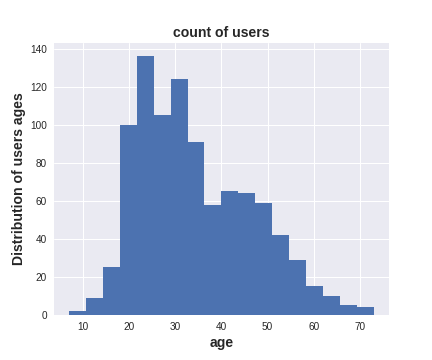
\includegraphics[width=\textwidth]{Bilder/age_dist.png}
\end{minipage}
\begin{minipage}[t]{0.33\textwidth}
	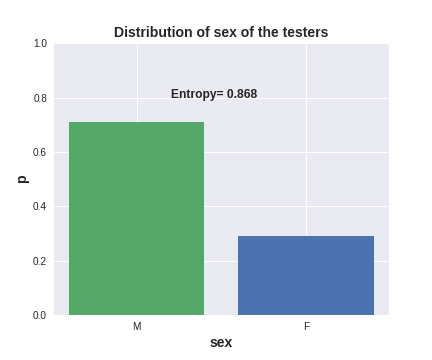
\includegraphics[width=\textwidth]{Bilder/sex_dist.png}
\end{minipage}
\begin{minipage}[t]{0.38\textwidth}
	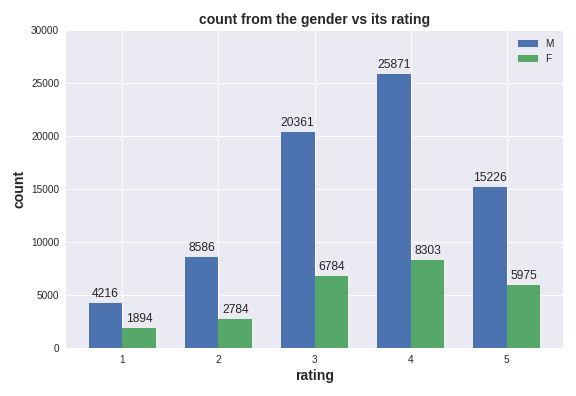
\includegraphics[width=\textwidth]{Bilder/sex_dist_rating.png}
\end{minipage}

%\begin{figure}[H]
%	\subfigure{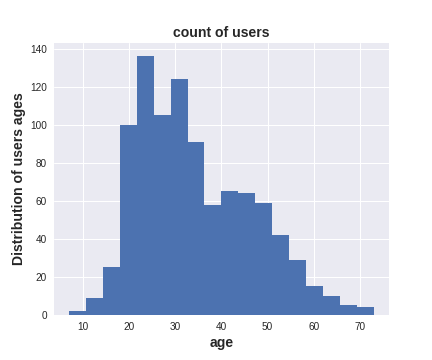
\includegraphics[width=0.49\textwidth]{Bilder/age_dist.png}}
%	\subfigure{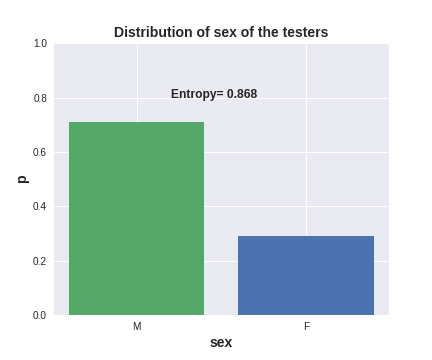
\includegraphics[width=0.49\textwidth]{Bilder/sex_dist.png}}
	%\caption{Titel unterm gesamten Bild}
%\end{figure}
\noindent
It is not a well distributed ages column. It would be better if it's better distributed. For example to increase the number of 38 age-old test users. On the other side the graph shows that there are roughly twice men as woman. This could be crucial for the rating for example for more women orientated films. Then the men would rate these movies worse than the women or in the other direction. On the right side we could definitely see the difference in the numbers of the rating from the Woman "F" and the men "M". The mean value of the rating from the men is 3.53 and for the women 3.52. That means that they choose wisely movies for women and also for men.
%Action	Adventure	Animation	Children	Comedy	Crime	Documentary	Drama	Fantasy	Film_Noir	Horror	Musical	Mystery	Romance	Sci_Fi	Thriller	War	Western	unknown
\begin{center}
\begin{tabular}{|p{2cm}|p{2cm}|p{2cm}|p{2cm}|p{2cm}|}
	\hline
	Children & Drama & Sci Fi & Thriller & Romance  \\ \hline
	-0.033961 & 0.034519 & 0.044447 & 0.030092 & -0.049035 \\
	\hline
\end{tabular}
\end{center}
This table shows the correlation between the sex or gender column with the different binomial classifiers form the movie. There is definetly no correlation between these values and the gender.
\begin{center}
	\begin{tabular}{|p{2cm}|p{2cm}|p{2cm}|p{2cm}|p{2cm}|}
		\hline
		Children & Drama & Sci Fi & Thriller & Romance  \\ \hline
		-0.043644 & 0.114006 & 0.010471 & -0.009802 & 0.040107 \\
		\hline
	\end{tabular}
\end{center}
Similar to the upper table there is also no correlation between in's binomial classifiers and the rating column.
%For the rating distribution there is a tendency for good rated films.

%The target for a regression and a classification task could be the "rating" column.\\\\
%For the classification there are multiple classes from (1-5) and the numbers itself for the regression. The input for the training of this model could be the columns to categorize the move. The problem is, that they are no clear correlation between thees columns $|C| = 0.11$ where $C$ is the correlation.
%\noindent
%In this graph the difference between the two genders in respect to the rating could better observe. 
%\begin{minipage}[t]{0.33\textwidth}
%	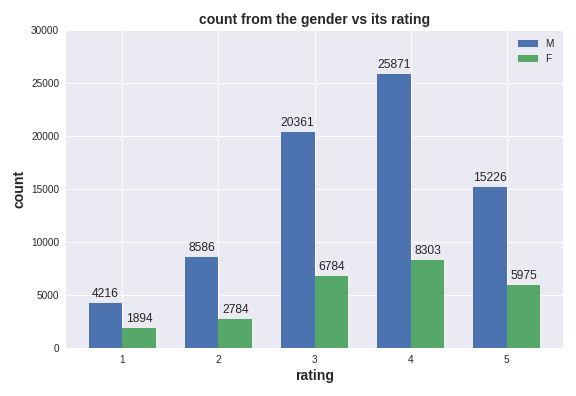
\includegraphics[width=\textwidth]{Bilder/sex_dist_rating.png}
%\end{minipage}

%\section{Potential ethical issues}
%In the user dataset there is the coloum "age" and "occupation". I think that are the only information, which is not ethnical correct. One solution that I could immagen is to divide the coloum "age" into four parts, such as "young", "medium", "adult" and "old".
%There are 21 different names in the coloum "occupation". Divide thees in different other names like "official", "private sector".


\end{document}